\chapter{Porovnávání dvou překladů}
Při zobrazování rozdílů dvou překladů můžeme zvýraznit slova či slovní spojení,
  která byla přeložena správně (potvrzené n-gramy),
  zlepšila nebo zhoršila překlad.
N-gramy, které byly přeloženy správně pouze v jednom z porovnávaných překladů,
  jsou zvýrazněny jako zlepšující.
Naopak n-gramy, které byly přeloženy špatně pouze v jednom z porovnávaných překladů,
  jsou zvýrazněny jako zhoršující. 

Druhou možností pro porovnávání překladů je zobrazení rozdílů porovnávaného překladu s referenčním překladem.
Pomocí této volby můžeme odhalit n-gramy,
  které se nacházejí na špatných pozicích ve větě,
  což může být způsobeno špatným slovosledem.

Při hledání potvrzených, zlepšujících nebo zhoršujících n-gramů nebo zobrazování diffu můžeme narazit na několik problémů,
  které si vysvětlíme v následující kapitole.
V závěru kapitoly si také ukážeme,
  jak bylo technicky realizováno zvýrazňování n-gramů pomocí HTML a CSS.

\section{Hledání potvrzených n-gramů}
Jelikož se ve větách mohou slova či tokeny libovolně opakovat,
  můžeme narazit na situaci,
  kdy budeme mít více kandidátů na potvrzený n-gram.
Člověk snadno rozezná,
  který n-gram je potvrzený,
  ale v dlouhých větách by to bylo časově náročné,
  proto jsme chtěli najít algoritmus,
  který by ze všech kandidátů na potvrzený n-gram našel ty,
  které jsou nejpravděpodobněji opravdu potvrzené n-gramy.

Pro znázornění hledání potvrzených n-gramů můžeme použít graf reprezentující porovnání dvou vět.
Tento graf se používá i pro výpočet diffu nebo LCS,
  které později budeme používat,
  proto si ho teď podrobněji popíšeme.
Každá hrana v tomto grafu odpovídá jednomu slovu z porovnávaných vět.
Horizontální čáry v grafu reprezentují slova, která jsou ve strojovém překladu navíc oproti překladu referenčnímu. 
Pro vertikální čáry to platí naopak, t.j. reprezentují slova, která jsou v referenčním překladu navíc oproti překladu referenčnímu.
Diagonalní čáry reprezentují shodu mezi referenčním a strojovým překladem.
Kandidáty na potvrzený n-gram si můžeme reprezentovat jako diagonální hrany v grafu,
  který představuje porovnání dvou vět.

\begin{figure}[h!]
\centering
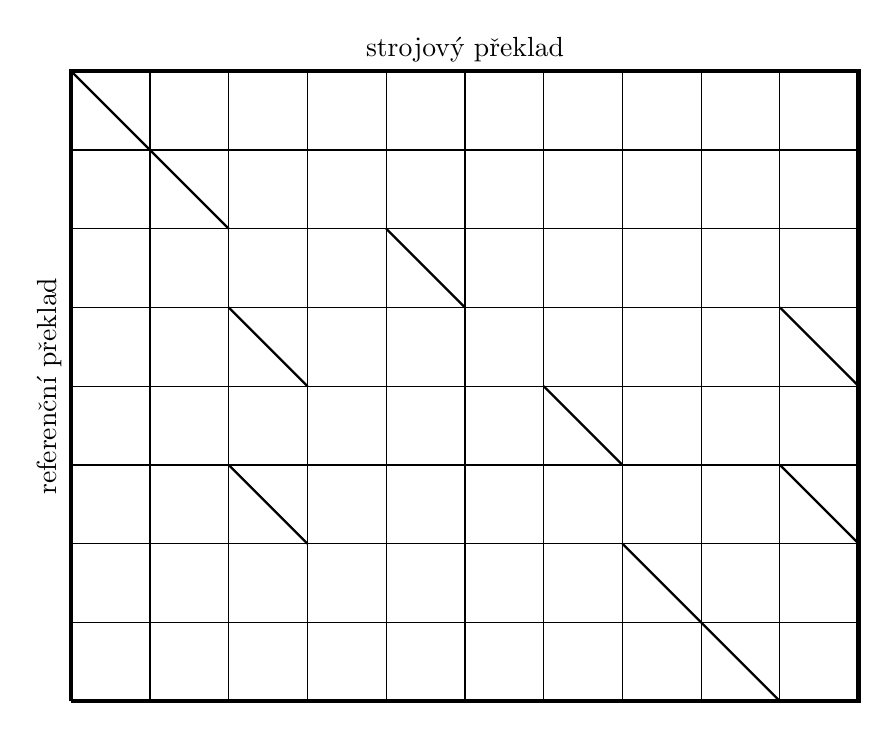
\begin{tikzpicture}
  \draw [ ultra thick ] (0,0)--(0,8)--(10,8)--(10,0)--(0,0);
  \draw (0,8)--(10,8) node [ midway, above ] { strojový překlad };
  \draw (0,0)--(0,8) node [ midway, above, rotate=90] { referenční překlad };
  \draw (0,1)--(10,1);
  \draw (0,2)--(10,2);
  \draw (0,3)--(10,3);
  \draw (0,4)--(10,4);
  \draw (0,5)--(10,5);
  \draw (0,6)--(10,6);
  \draw (0,7)--(10,7);
  \draw (1,0)--(1,8);
  \draw (2,0)--(2,8);
  \draw (3,0)--(3,8);
  \draw (4,0)--(4,8);
  \draw (5,0)--(5,8);
  \draw (6,0)--(6,8);
  \draw (7,0)--(7,8);
  \draw (8,0)--(8,8);
  \draw (9,0)--(9,8);
  \draw [thick] (0,8)--(2,6);
  \draw [thick] (4,6)--(5,5);
  \draw [thick] (6,4)--(7,3);
  \draw [thick] (2,5)--(3,4);
  \draw [thick] (9,5)--(10,4);
  \draw [thick] (2,3)--(3,2);
  \draw [thick] (9,3)--(10,2);
  \draw [thick] (7,2)--(9,0);
\end{tikzpicture}
\end{figure}

V případě,
  že počet kandidátů na potvrzený n-gram se rovná počtu potvrzených n-gramů,
  je řešení našeho problému jednoduché.
V grafu to odpovídá situaci,
  kdy se v řádku a sloupci nachází stejný počet diagonálních čar.
V případě,
  že se nějaký potvrzený n-gram vyskytuje vícekrát,
  použijeme vždy prvního ještě nepoužitého kandidáta.
Všichni kandidáti na potvrzený n-gram jsou potvrzené n-gramy,
  a tak je můžeme patřičně zvýraznit.
V našich obrázcích budeme zvýrazňovat potvrzené n-gramy červenou barvou.

\begin{figure}[h!]
\centering
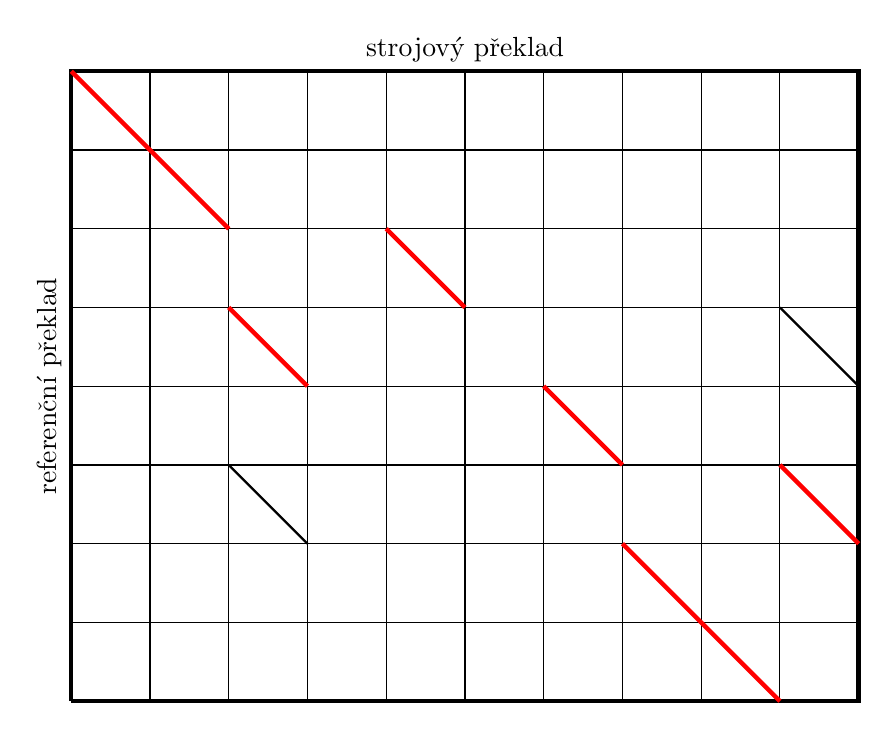
\begin{tikzpicture}
  \draw [ ultra thick ] (0,0)--(0,8)--(10,8)--(10,0)--(0,0);
  \draw (0,8)--(10,8) node [ midway, above ] { strojový překlad };
  \draw (0,0)--(0,8) node [ midway, above, rotate=90] { referenční překlad };
  \draw (0,1)--(10,1);
  \draw (0,2)--(10,2);
  \draw (0,3)--(10,3);
  \draw (0,4)--(10,4);
  \draw (0,5)--(10,5);
  \draw (0,6)--(10,6);
  \draw (0,7)--(10,7);
  \draw (1,0)--(1,8);
  \draw (2,0)--(2,8);
  \draw (3,0)--(3,8);
  \draw (4,0)--(4,8);
  \draw (5,0)--(5,8);
  \draw (6,0)--(6,8);
  \draw (7,0)--(7,8);
  \draw (8,0)--(8,8);
  \draw (9,0)--(9,8);
  \draw [ultra thick, red] (0,8)--(2,6);
  \draw [ultra thick, red] (4,6)--(5,5);
  \draw [ultra thick, red] (6,4)--(7,3);
  \draw [ultra thick, red] (2,5)--(3,4);
  \draw [ultra thick, red] (9,3)--(10,2);
  \draw [ultra thick, red] (7,2)--(9,0);
  \draw [thick] (9,5)--(10,4);
  \draw [thick] (2,3)--(3,2);
\end{tikzpicture}
\end{figure}

Těžší situace nastane,
  když si budeme muset z kadidátů vybírat.

\begin{figure}[h!]
\centering
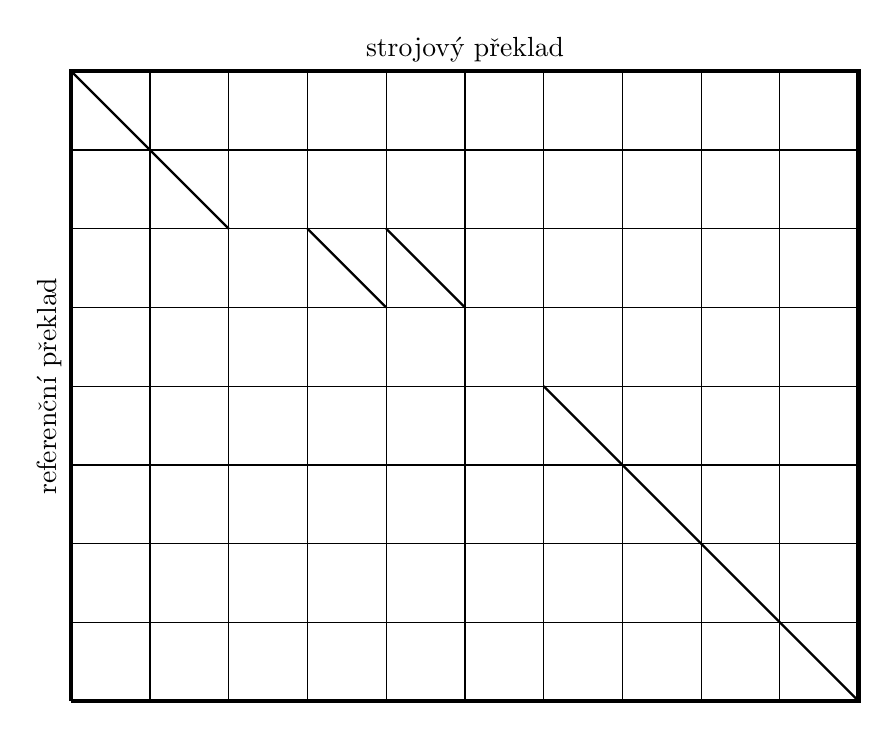
\begin{tikzpicture}
  \draw [ ultra thick ] (0,0)--(0,8)--(10,8)--(10,0)--(0,0);
  \draw (0,8)--(10,8) node [ midway, above ] { strojový překlad };
  \draw (0,0)--(0,8) node [ midway, above, rotate=90] { referenční překlad };
  \draw (0,1)--(10,1);
  \draw (0,2)--(10,2);
  \draw (0,3)--(10,3);
  \draw (0,4)--(10,4);
  \draw (0,5)--(10,5);
  \draw (0,6)--(10,6);
  \draw (0,7)--(10,7);
  \draw (1,0)--(1,8);
  \draw (2,0)--(2,8);
  \draw (3,0)--(3,8);
  \draw (4,0)--(4,8);
  \draw (5,0)--(5,8);
  \draw (6,0)--(6,8);
  \draw (7,0)--(7,8);
  \draw (8,0)--(8,8);
  \draw (9,0)--(9,8);
  \draw [thick] (0,8)--(2,6);
  \draw [thick] (4,6)--(5,5);
  \draw [thick] (6,4)--(10,0);
  \draw [thick] (3,6)--(4,5);
\end{tikzpicture}
\end{figure}

To je poměrně častý jev,
  který je k vidění např. u předložek, spojek nebo interpunkce.
V takovéto situaci chceme vybrat takové kandidáty,
  kteří se nacházejí v nejdelších možných potvrzených n-gramech.
K hledaní kandidátů nacházejících se v nejdelších potvrzených n-gramech je možné použít algoritmus LCS.
Nejdelší společná podposloupnost leží na nejkratší monotonní cestě v grafu,
  která vede z levého horního do pravého dolního rohu.
V obrázku budeme znázorňovat tuto cestu zelenou barvou.
Všichni kandidáti, kteří se nacházejí na této cestě,
  určitě patří mezi potvrzené n-gramy.
To plyne přímo z definice nejdelší společné podposloupnosti.

\begin{figure}[h!]
\centering
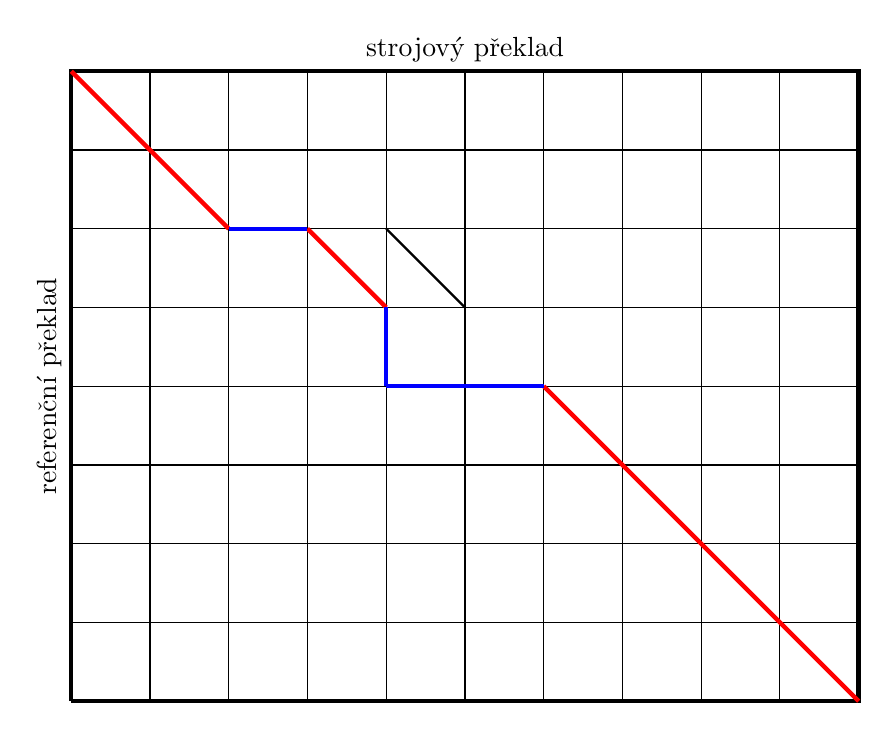
\begin{tikzpicture}
  \draw [ ultra thick ] (0,0)--(0,8)--(10,8)--(10,0)--(0,0);
  \draw (0,8)--(10,8) node [ midway, above ] { strojový překlad };
  \draw (0,0)--(0,8) node [ midway, above, rotate=90] { referenční překlad };
  \draw (0,1)--(10,1);
  \draw (0,2)--(10,2);
  \draw (0,3)--(10,3);
  \draw (0,4)--(10,4);
  \draw (0,5)--(10,5);
  \draw (0,6)--(10,6);
  \draw (0,7)--(10,7);
  \draw (1,0)--(1,8);
  \draw (2,0)--(2,8);
  \draw (3,0)--(3,8);
  \draw (4,0)--(4,8);
  \draw (5,0)--(5,8);
  \draw (6,0)--(6,8);
  \draw (7,0)--(7,8);
  \draw (8,0)--(8,8);
  \draw (9,0)--(9,8);
  \draw [ultra thick, red] (0,8)--(2,6);
  \draw [ultra thick, red] (3,6)--(4,5);
  \draw [ultra thick, red] (6,4)--(10,0);
  \draw [thick] (4,6)--(5,5);

  \draw [ultra thick, blue] (2,6)--(3,6);
  \draw [ultra thick, blue] (4,5)--(4,4);
  \draw [ultra thick, blue] (4,4)--(6,4);
\end{tikzpicture}
\end{figure}

Tímto postupem jsme schopní nalézt pozice všech potvrzených n-gramů,
  které se nacházejí v nejdelší společné podposloupnosti.
Ale ne všechny potvrzené n-gramy se zde musí nacházet,
  může se stát,
  že např. bylo změněno pořadí slov v překladu a potvrzený n-gram se nenachází v nejdelší společné podposloupnosti.

\begin{figure}[h!]
\centering
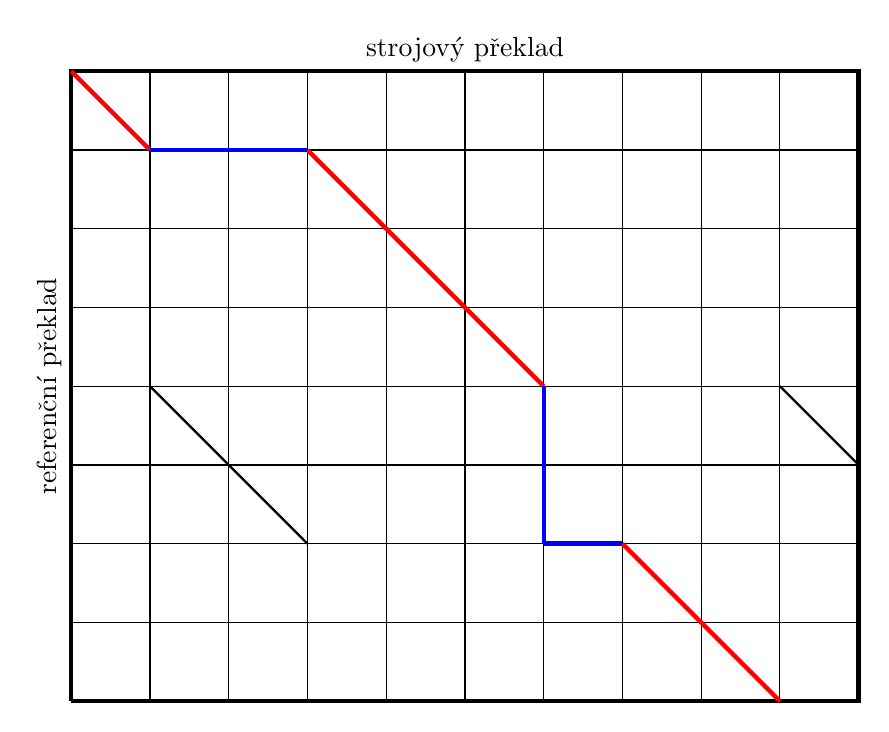
\begin{tikzpicture}
  \draw [ ultra thick ] (0,0)--(0,8)--(10,8)--(10,0)--(0,0);
  \draw (0,8)--(10,8) node [ midway, above ] { strojový překlad };
  \draw (0,0)--(0,8) node [ midway, above, rotate=90] { referenční překlad };
  \draw (0,1)--(10,1);
  \draw (0,2)--(10,2);
  \draw (0,3)--(10,3);
  \draw (0,4)--(10,4);
  \draw (0,5)--(10,5);
  \draw (0,6)--(10,6);
  \draw (0,7)--(10,7);
  \draw (1,0)--(1,8);
  \draw (2,0)--(2,8);
  \draw (3,0)--(3,8);
  \draw (4,0)--(4,8);
  \draw (5,0)--(5,8);
  \draw (6,0)--(6,8);
  \draw (7,0)--(7,8);
  \draw (8,0)--(8,8);
  \draw (9,0)--(9,8);
  \draw [ultra thick, red] (0,8)--(1,7);
  \draw [ultra thick, red] (3,7)--(6,4);
  \draw [ultra thick, red] (7,2)--(9,0);

  \draw [ultra thick, blue] (1,7)--(3,7);
  \draw [ultra thick, blue] (6,4)--(6,2);
  \draw [ultra thick, blue] (6,2)--(7,2);

  \draw [thick] (1,4)--(3,2);

  \draw [thick] (9,4)--(10,3);
\end{tikzpicture}
\end{figure}

I tato situace může nastat poměrně často,
  proto jsme museli vymyslet způsob,
  jak z kandidátů potvrzených n-gramů,
  kteří se nacházejí mimo nejdelší společnou podposloupnost,
  vybereme potvrzené n-gramy. 

\begin{figure}[h!]
\centering
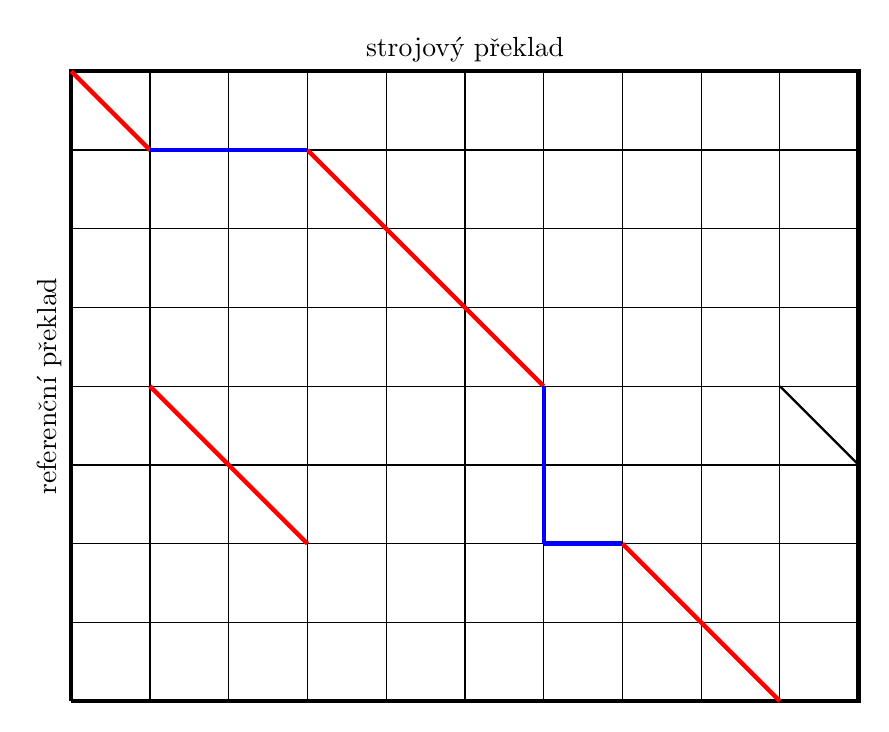
\begin{tikzpicture}
  \draw [ ultra thick ] (0,0)--(0,8)--(10,8)--(10,0)--(0,0);
  \draw (0,8)--(10,8) node [ midway, above ] { strojový překlad };
  \draw (0,0)--(0,8) node [ midway, above, rotate=90] { referenční překlad };
  \draw (0,1)--(10,1);
  \draw (0,2)--(10,2);
  \draw (0,3)--(10,3);
  \draw (0,4)--(10,4);
  \draw (0,5)--(10,5);
  \draw (0,6)--(10,6);
  \draw (0,7)--(10,7);
  \draw (1,0)--(1,8);
  \draw (2,0)--(2,8);
  \draw (3,0)--(3,8);
  \draw (4,0)--(4,8);
  \draw (5,0)--(5,8);
  \draw (6,0)--(6,8);
  \draw (7,0)--(7,8);
  \draw (8,0)--(8,8);
  \draw (9,0)--(9,8);
  \draw [ultra thick, red] (0,8)--(1,7);
  \draw [ultra thick, red] (3,7)--(6,4);
  \draw [ultra thick, red] (7,2)--(9,0);

  \draw [ultra thick, blue] (1,7)--(3,7);
  \draw [ultra thick, blue] (6,4)--(6,2);
  \draw [ultra thick, blue] (6,2)--(7,2);

  \draw [ultra thick, red] (1,4)--(3,2);

  \draw [thick] (9,4)--(10,3);
\end{tikzpicture}
\end{figure}

Při vymýšlení algoritmu pro řešení této situace jsme použili stejný předpoklad jako v minulém případě.
T.j. že z kadidátů potvrzených n-gramů vybíráme vždy ty kandidáty,
  kteří se nacházejí uvnitř nejdelších potvrzených n-gramů.
Pro každý token si můžeme počítat skóre,
  v kolika kandidátech potvrzených n-gramů a již potvrzených n-gramech se nachází.
Z kadidátů na potvrzený n-gram pak vybereme ty,
  které mají největší skóre n-gramu,
  které se spočítá jako součet skóre tokenů v n-gramu.
Abychom nadále nezvýhodňovali kandidáty,
  kteří byli součástí delších nezvolených kandidátů,
  musíme po každé volbě potvrzených n-gramů upravit skóre u kandidátů,
  kteří nebyli zvoleni za potvrzené n-gramy.
  
Abychom mohli zkombinovat oba dva přístupy do jednoho algoritmu a
  nemuseli jsme zvlášť řešit jednotlivé případy,
  přidali jsme bonifikaci pro tokeny,
  které se nacházejí v nejdelší společné podposloupnosti.
Tyto tokeny budou mít vždy vyšší skóre než jejich konkurenti,
  a proto nemůže dojít k situaci,
  že by token ležící v nejdelší společené podposloupnosti nebyl částí potvrzeného n-gramu.
Nalezení potvrzených n-gramů pak můžeme provést pouze pomocí počítání skóre.


Avšak i kombinace těchto dvou přístupů nemusí vždy fungovat.
Jelikož počítáme s n-gramy pouze do délky čtyř tokenů,
  potvrzené n-gramy,
  které se nenacházejí v nejdelší společné podposloupnosti a jsou delší než sedm tokenů,
  nemusejí být správně označeny za potvrzené.
U takovýchto n-gramů záleží pouze na pořadí, v jakém se ve větě vyskytují.
Část n-gramu,
  který se ve větě vyskytne dříve,
  bude prohlášen za potvrzený n-gram.

V praxi se ale tyto případy moc nevyskytují -
  nestává se často, že by se ve větě nacházelo více kandidátů pro n-gram délky vyšší než sedm tokenů,
  proto by měl náš algoritmus ve většině případů fungovat dobře.


\section{Počítání diffu mezi dvěma překlady}
Pro počítání diffu mezi dvěma překlady můžeme použít stejný algoritmus,
  který jsme používali k hledání nejdelší společné podposloupnosti dvou překladů.
Diff je stejně jako nejdelší společná podposloupnost reprezentován nejkratší monotonní cestou vedoucí z levého horního do pravého dolního rohu.
Změna je pouze v tom, že horizontální hrany ležící na této cestě odpovídají tokenům,
  které se nacházejí pouze ve strojovém překladu.
V diagramu je budeme označovat modrou barvou.
Vertikální hrany ležící na cestě reprezentující nejdelší společnou podposloupnost odpovídají tokenům,
  které se nacházejí pouze v referenčním překladu.
V diagramu je budeme označovat červenou barvou.
Diagonální hrany ležící na výše definované cestě reprezentují tokeny,
  které se nacházejí v obou porovnávaných překladech.
V diagramu je budeme označovat zelenou barvou.
Z takto obarvené cesty můžeme zjistit rozdíl mezi porovnávanými větami
  a na jeho základě můžeme zobrazit rozdíl ve webovém prostředí.

\begin{figure}[h!]
\centering
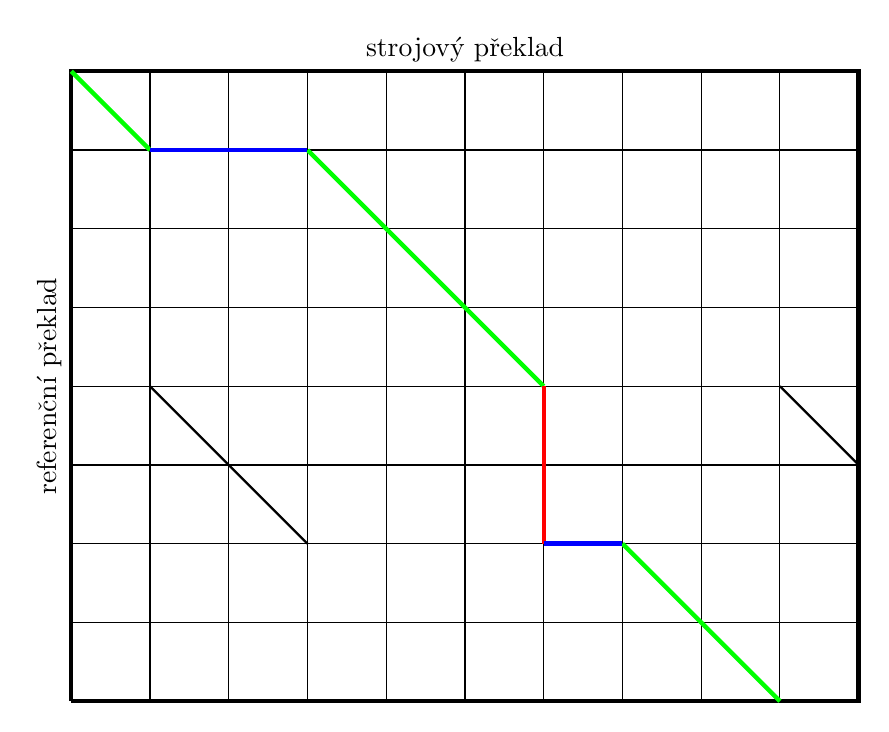
\begin{tikzpicture}
  \draw [ ultra thick ] (0,0)--(0,8)--(10,8)--(10,0)--(0,0);
  \draw (0,8)--(10,8) node [ midway, above ] { strojový překlad };
  \draw (0,0)--(0,8) node [ midway, above, rotate=90] { referenční překlad };
  \draw (0,1)--(10,1);
  \draw (0,2)--(10,2);
  \draw (0,3)--(10,3);
  \draw (0,4)--(10,4);
  \draw (0,5)--(10,5);
  \draw (0,6)--(10,6);
  \draw (0,7)--(10,7);
  \draw (1,0)--(1,8);
  \draw (2,0)--(2,8);
  \draw (3,0)--(3,8);
  \draw (4,0)--(4,8);
  \draw (5,0)--(5,8);
  \draw (6,0)--(6,8);
  \draw (7,0)--(7,8);
  \draw (8,0)--(8,8);
  \draw (9,0)--(9,8);
  \draw [ultra thick, green] (0,8)--(1,7);
  \draw [ultra thick, green] (3,7)--(6,4);
  \draw [ultra thick, green] (7,2)--(9,0);

  \draw [ultra thick, blue] (1,7)--(3,7);
  \draw [ultra thick, red] (6,4)--(6,2);
  \draw [ultra thick, blue] (6,2)--(7,2);

  \draw [thick] (1,4)--(3,2);
  \draw [thick] (9,4)--(10,3);
\end{tikzpicture}
\end{figure}


\section{Zobrazení potvrzených n-gramů a diffu pomocí}
Pro správné zobrazení potvrzených n-gramů a diffu je potřeba,
  abychom mohli každému tokenu říci,
  jestli se nachází v nějakém potvrzeném n-gramu nebo jestli byl do věty přidán.
Zároveň s touto informací chceme,
  aby jednotlivá zvýraznění bylo možné libovolně kombinovat.
Technicky tento problém byl vyřešen pomoci CSS tříd,
  kdy každému tokenu byly přiřazeny třídy v závislosti na informacích,
  které jsme si vypočítali pomocí výše uvedených postupů.
Zapnutí a vypnutí jednotlivých kombinací je pak otázkou přiřazení příslušné třídy kořenovému elementu,
  v kterém se nacházejí všechny věty.
Přehlednost těchto kombinací nemusí být vždy zcela ideální, 
  proto jsme se snažili udělat jednotlivá zvýraznění tak,
  aby byla co nejjednodušeji modifikovatelná.
Každý typ zvýraznění tak má vlastní selektor,
  pomocí kterého může zvýraznění v CSS upravit.

